%% ============================================================
%% FlowPMO — IEEE Conference Paper (IEEEtran)
%% ============================================================
\documentclass[conference]{IEEEtran}

\usepackage{graphicx}
\usepackage{booktabs}
\usepackage{multirow}
\usepackage{amsmath,amssymb}
\usepackage{hyperref}
\usepackage{xcolor}
\usepackage{array}
\usepackage{tabularx}
\usepackage{microtype}

\hypersetup{
  colorlinks=true,
  linkcolor=blue!60!black,
  citecolor=blue!60!black,
  urlcolor=blue!60!black
}

% ============================================================
\title{FlowPMO: Operationalizing Multidimensional Developer\\
       Productivity with Absolute Benchmark Normalization}

\author{
  \IEEEauthorblockN{Rodrigo Almeida de Oliveira}
  \IEEEauthorblockA{Flow Engineering Research Group\\
  \texttt{rodrigoalmeidadeoliveira@gmail.com}}
}

\begin{document}
\maketitle

% ============================================================
\begin{abstract}
Measuring developer productivity remains one of the most contested challenges in
software engineering management. Widely adopted proxies --- lines of code, commit
frequency, and velocity points --- are uni-dimensional and susceptible to gaming.
This paper presents \textbf{FlowPMO}, an open-source Plotly/Dash dashboard that
operationalizes developer productivity across five SPACE-inspired dimensions:
Delivery Output, Flow Efficiency, Review Quality, Process Conformance, and
Anti-Rework, each normalized against absolute, literature-grounded benchmarks.
Beyond the five radar dimensions, FlowPMO introduces three composite indices:
the \textbf{IED} (weighted NDS+EEE+VEL+QUA composite), the \textbf{IEF}
(delivery-only NDS+EEE subindex), and the \textbf{IEF--IED Divergence~($\Delta$)},
a diagnostic signal flagging developers whose velocity or quality penalty distorts
their delivery signal.
Three measurement validity corrections are also introduced: \textbf{FE~Ajustada}
(cross-period WIP saturation fix), \textbf{role-fair NDS} (role-specific P75),
and \textbf{Bayesian QUA smoothing} (Beta prior $\alpha=0.5$, $\beta=9.5$).
A team-level \textbf{ICC} (Herfindahl-Hirschman) quantifies commit-concentration
risk per organizational unit.
Evaluation on a reproducible synthetic dataset of 28~developers (5~teams, Q3~2024,
seed=42) shows that: role-specific P75 reduces the IED gap between Tech Leads and
individual contributors from $-16.9$ to $-3.7$~points; Bayesian smoothing raises
QUA by up to 47.5~pp for extreme low-sample cases; and IEF--IED divergence
exceeds 15~points for 3 of 28~developers (10.7\%), each requiring a qualitatively
different coaching intervention.
\end{abstract}

\begin{IEEEkeywords}
developer productivity, SPACE framework, benchmark normalization, composite index,
Bayesian shrinkage, flow efficiency, process mining, knowledge concentration
\end{IEEEkeywords}

% ============================================================
\section{Introduction}
\label{sec:intro}
% ============================================================

Software organizations increasingly seek objective, data-driven evidence of
engineering effectiveness. Yet the choice of productivity proxy shapes
organizational behavior profoundly: when a single metric becomes a target, it
ceases to be a good measure~\cite{demarco1999}. Commit frequency rewards small
commits; velocity points reward estimation inflation; lines of code reward
verbosity. None is intrinsically wrong, but each is dangerously incomplete in
isolation.

The SPACE framework~\cite{forsgren2021} provides a principled taxonomy across
five dimensions: Satisfaction, Performance, Activity, Collaboration, and
Efficiency. SPACE explicitly cautions against reducing productivity to any single
dimension but does not prescribe how to operationalize, normalize, or compose
metrics into a practitioner dashboard.

FlowPMO fills this gap. It is an open-source Python/Dash
dashboard\footnote{Repository: \url{https://github.com/rodrigoalmeidadeoliveira/flow-pmo}}
that ingests Jira and Bitbucket telemetry and produces per-developer productivity
profiles aligned with five SPACE-inspired dimensions. A second gap addressed here
is \emph{measurement validity at the margins}: flow efficiency inflated by
cross-period WIP carry-over, quality scores that collapse to zero for one defect
in one delivery, and delivery benchmarks that structurally penalize Tech Leads.

\subsection*{Contributions}

This paper makes ten contributions:
\begin{enumerate}
  \item Five-dimensional productivity framework with absolute benchmark normalization.
  \item Score Benchmark (SB): euclidean distance to ideal $[100,\ldots,100]$.
  \item Process-mining integration for conformance and rework at individual level.
  \item Anonymized production-data validation (LGPD-safe).
  \item \textbf{IED} --- composite index NDS+EEE+VEL+QUA (0.40/0.30/0.20/0.10).
  \item \textbf{IEF} and \textbf{IEF--IED Divergence ($\Delta$)} --- delivery subindex + diagnostic signal.
  \item \textbf{Role-fair NDS}: role-specific P75 eliminates structural TL penalty.
  \item \textbf{QUA Bayesian shrinkage}: Beta(0.5, 9.5) prior for low-sample correction.
  \item \textbf{FE~Ajustada}: cross-period WIP correction for Flow Efficiency.
  \item \textbf{ICC}: Herfindahl-Hirschman commit-concentration risk per team.
\end{enumerate}

\subsection*{Research Questions}

\begin{itemize}
  \item \textbf{RQ1}: Does IED capture productivity variance invisible to single metrics?
  \item \textbf{RQ2}: How does Flow Efficiency relate to conformance, rework, and WIP?
  \item \textbf{RQ3}: How does role-specific P75 affect the IED gap between Tech Leads and Devs?
  \item \textbf{RQ4}: Does IEF--IED divergence identify actionable coaching signals beyond either index alone?
\end{itemize}

% ============================================================
\section{Background and Related Work}
\label{sec:background}
% ============================================================

\subsection{Developer Productivity Measurement}

Early productivity measurement focused on LOC and function
points~\cite{fenton1997}, both suffering from incentive misalignment.
The SPACE framework~\cite{forsgren2021} argues that no single dimension captures
the latent productivity construct and that organizations should measure at least
one indicator from each of the five SPACE categories.
Jørgensen~\cite{jorgensen2014} finds that multi-dimensional schemes predict team
performance significantly better (effect size $d=0.42$) than uni-dimensional ones.

\subsection{DORA Metrics and Flow Framework}

The DORA program~\cite{forsgren2018} identified four team-level software delivery
metrics as organizational performance predictors. Anderson~\cite{anderson2010}
applied flow efficiency ($\geq 80\%$) to software Kanban.
A well-known pathology of individual-level flow efficiency is \emph{cross-period
inflation}: items delivered from a prior period inflate the numerator without a
corresponding denominator entry. The FE~Ajustada correction
(Section~\ref{sec:fe_ajustada}) addresses this.

\subsection{Process Mining in Software Engineering}

Process mining~\cite{vanderaalst2016} enables conformance checking against
normative workflow models. Caldeira et al.~\cite{caldeira2019} applied conformance
checking to Jira logs, showing that deviations correlate with defect density and
cycle-time inflation. FlowPMO adapts these techniques to produce individual-level
conformance and rework scores.

\subsection{Rework and Quality Metrics}

Shah et al.~\cite{shah2023} found that rework rates above 25\% accumulate
technical debt at twice the rate of teams below 15\%. Nogueira and
Rela~\cite{nogueira2023} report that pipeline success rates below 70\% predict
elevated defect escape rates.

\subsection{Small-Sample Estimation and Bayesian Methods}

A developer with one defect in one delivery receives QUA~$=0$; with zero defects in
one delivery, QUA~$=100$. Gelman et al.~\cite{gelman2013} provide the theoretical
basis for Bayesian shrinkage via a conjugate Beta-Binomial prior. FlowPMO applies
a Beta(0.5, 9.5) prior --- corresponding to a prior failure rate of 5\% with
effective sample size 10 --- to regularize QUA in low-sample scenarios.

\subsection{Knowledge Concentration and Bus Factor}

Ricca et al.~\cite{ricca2019} quantify truck factor as the number of developers
whose removal causes critical knowledge loss. The Herfindahl-Hirschman Index
(HHI)~\cite{doj2010} provides a continuous analogue:
$\text{HHI} = \sum_i s_i^2$, where $s_i$ is developer $i$'s share of team
commits. The U.S.~DOJ classifies $\text{HHI} > 0.25$ as highly concentrated.
FlowPMO adapts this threshold as the commit-concentration risk signal (ICC).

% ============================================================
\section{The FlowPMO Framework}
\label{sec:framework}
% ============================================================

\subsection{Architecture}

FlowPMO integrates three primary data sources into a Plotly/Dash dashboard:
Jira CSV exports (issue lifecycle events), Bitbucket activity logs (commits, PRs,
reviews), and an optional process-mining Excel report. The processing pipeline has
five stages: (1)~raw ingestion and schema normalization; (2)~developer-period
aggregation; (3)~derived metric computation; (4)~benchmark normalization and radar
score computation; (5)~dashboard rendering.

\subsection{Five Productivity Dimensions}

Table~\ref{tab:dimensions} summarizes the five dimensions, primary metrics,
benchmarks, and references.

\begin{table}[htbp]
  \centering
  \caption{FlowPMO productivity dimensions.}
  \label{tab:dimensions}
  \small
  \setlength{\tabcolsep}{4pt}
  \begin{tabular}{clp{2.2cm}p{1.5cm}c}
    \toprule
    \textbf{\#} & \textbf{Dimension} & \textbf{Metric} & \textbf{Benchmark} & \textbf{Ref.} \\
    \midrule
    D1 & Delivery  & Score Complexity / P75(role) & P75 role & \cite{jorgensen2014} \\
    D2 & Flow Eff. & FE Ajustada (\%) & $\geq$80\% & \cite{anderson2010} \\
    D3 & Review    & Approvals / reviews & $\geq$70\% & \cite{forsgren2021} \\
    D4 & Conformance & Conformance \% & $\geq$75\% & \cite{caldeira2019} \\
    D5 & Anti-Rework & $100-$Rework~\% & $\leq$20\% rework & \cite{shah2023} \\
    \bottomrule
  \end{tabular}
\end{table}

\textbf{Score Complexity} weights delivered items by story-point bucket: no
estimate~$=0.5$; 1--3~SP~$=1.0$; 5--8~SP~$=2.0$; 13+~SP~$=3.0$. T-shirt sizes
are equalized via functional-weight mapping~\cite{kitchenham2004}.

\subsection{Absolute Benchmark Normalization}

Each dimension score $d_i$ is normalized against benchmark $\beta_i$:

\begin{equation}
  \hat{d}_i = \min\!\left(\frac{d_i}{\beta_i} \times 100,\; 100\right)
  \label{eq:norm}
\end{equation}

This avoids the \emph{rank-collapse} problem of z-score normalization in small
homogeneous teams. The sole exception is D1, where P75 is role-specific
(Section~\ref{sec:role_nds}).

\subsection{Score Benchmark Composite Index}

The Score Benchmark (SB) is the complement of the normalized euclidean distance
from the developer's five-dimensional profile $\mathbf{r}$ to the ideal
$\mathbf{v}^* = [100,100,100,100,100]$:

\begin{equation}
  \text{SB} = 100 - \frac{\left\|\mathbf{r} - \mathbf{v}^*\right\|_2}{\sqrt{5}\times 100} \times 100
  \label{eq:sb}
\end{equation}

SB is bounded in $[0,100]$ by construction. Equal dimension weights are a
deliberate default; organizations may substitute a weighted distance.

\subsection{FE Ajustada --- Cross-Period WIP Correction}
\label{sec:fe_ajustada}

Raw FE $= \text{items\_delivered} / \text{items\_pulled} \times 100$ can exceed
100\% when items pulled in a prior period are delivered in the current one. The
corrected denominator includes \emph{WIP~Inicio~Periodo}: items where
$\texttt{DataInProgress} < t_\text{start}$ and $(\texttt{DataDone} \geq
t_\text{start}$ or $\texttt{DataDone}~=~\text{null})$:

\begin{equation}
  \text{FE\_ajustada} = \min\!\left(
    \frac{\text{items\_delivered}}{\text{items\_pulled} + \text{wip\_inicio}},\;
    1 \right) \times 100
  \label{eq:fe_adj}
\end{equation}

Both raw FE (for traceability) and FE\_ajustada are retained.
The \texttt{\_rb\_flow} radar dimension and the EEE fallback in the IED
use FE\_ajustada exclusively.

\subsection{\'Indice de Entrega do Desenvolvedor (IED)}
\label{sec:ied}

The IED is a four-component weighted composite:

\begin{equation}
  \text{IED} = 0.40\cdot\text{NDS} + 0.30\cdot\text{EEE}
             + 0.20\cdot\text{VEL} + 0.10\cdot\text{QUA}
  \label{eq:ied}
\end{equation}

\begin{itemize}
  \item \textbf{NDS} --- Score~Complexity / P75(role) $\times$ 100, clipped to
    $[0,100]$. Delivery volume adjusted for complexity vs.\ role-specific P75.
  \item \textbf{EEE} --- Score~Complexity\_delivered / Score~Complexity\_pulled
    $\times$ 100. Completion rate of committed work; falls back to FE\_ajustada
    when the pulled complexity is zero. Source: Kitchenham \& Mendes~\cite{kitchenham2004}.
  \item \textbf{VEL} --- $\text{Median\_LT\_group} / \text{LT\_dev} \times 100$.
    Lower lead time $=$ higher VEL. When LT $=$ 0, fallback $=$ group median VEL
    (not a fixed constant). Source: Flournoy et al.~\cite{flournoy2025}.
  \item \textbf{QUA} --- Bayesian-smoothed quality (Section~\ref{sec:bayes_qua}).
\end{itemize}

IED thresholds: Excellent $\geq 85$ | Good $\geq 70$ | Regular $\geq 50$ |
Below Expected $\geq 30$ | Critical $< 30$.

\subsection{\'Indice de Entrega Focado (IEF) and Divergence}
\label{sec:ief}

The IEF isolates delivery capacity from process penalties:

\begin{equation}
  \text{IEF} = 0.70\cdot\text{NDS} + 0.30\cdot\text{EEE}
  \label{eq:ief}
\end{equation}

The \textbf{IEF--IED Divergence} $\Delta = |\text{IEF} - \text{IED}|$ is a
diagnostic signal:

\begin{itemize}
  \item $\text{IEF} > \text{IED}$: VEL or QUA penalty suppresses IED
    below delivery capacity.
  \item $\text{IEF} < \text{IED}$: excellent VEL or QUA elevates IED above
    delivery throughput signal.
\end{itemize}

$\Delta > 15$ is flagged as actionable, directing coaching toward the specific
penalty dimension rather than the aggregate composite.

\subsection{Role-Fair NDS Benchmarking}
\label{sec:role_nds}

In the baseline formulation, NDS uses the population-wide P75 as its benchmark.
With P75$_\text{global} = 21.25$, a Tech Lead with
Score~Complexity~$=10$ receives NDS~$=47.1$; the same developer benchmarked
against TL-group P75~$=13.0$ receives NDS~$=76.9$ ($+29.8$~pp). This correction
reflects that TL responsibilities reduce item delivery time without indicating
underperformance.

The implementation uses
$\texttt{groupby(}\textit{role}\texttt{).quantile(0.75)}$, with fallback to
population P75 when the cohort contains only one role.

\subsection{QUA Bayesian Smoothing}
\label{sec:bayes_qua}

Raw QUA~$= (1 - \text{defects}/\text{deliveries}) \times 100$ is highly
unstable for small delivery counts. FlowPMO applies a Beta-Binomial conjugate
prior:

\begin{equation}
  \hat{p}_\text{fail} = \frac{\text{defects} + \alpha}{\text{deliveries} + \alpha + \beta}
  \label{eq:bayes}
\end{equation}

\begin{equation}
  \text{QUA} = (1 - \hat{p}_\text{fail}) \times 100
  \label{eq:qua}
\end{equation}

with $\alpha = 0.5$, $\beta = 9.5$ (prior failure rate 5\%, effective sample
size 10). As deliveries grow, the posterior converges to the empirical rate and
the correction vanishes. Source: Gelman et al.~\cite{gelman2013}.

\subsection{Estimation Coverage Rate (ECR)}

\begin{equation}
  \text{ECR} = \left(1 - \frac{n_\text{inferred}}{n_\text{pulled}}\right) \times 100
\end{equation}

When ECR $< 50\%$, NDS and EEE rely predominantly on statistically inferred
weights. A \textbf{Confiança~IED} badge ($\triangle\,$ECR${<}50\%$ / $\checkmark$)
alerts managers without invalidating the score.
Source: Kitchenham \& Mendes~\cite{kitchenham2004}.

\subsection{ICC --- Knowledge Concentration Risk}

\begin{equation}
  \text{ICC} = \sum_i \left(\frac{\text{commits}_i}{\text{commits}_\text{team}}\right)^2
\end{equation}

\begin{equation}
  \text{ICC}_\text{norm} = \frac{\text{ICC} - 1/N}{1 - 1/N}, \quad N > 1
\end{equation}

ICC~$=1/N$ indicates perfect distribution; ICC~$\to 1$ indicates full
concentration. ICC~$> 0.25$ (raw) is flagged as ``Concentrated.''
$\text{ICC}_\text{norm}$ corrects for team-size bias when comparing teams of
different sizes.
Source: Ricca et al.~\cite{ricca2019}; U.S.~DOJ HHI standard~\cite{doj2010}.

% ============================================================
\section{Evaluation Design}
\label{sec:evaluation}
% ============================================================

\subsection{Synthetic Dataset}

We evaluate the framework on a reproducible synthetic dataset of 28~developers
across 5~teams for Q3~2024 ($\texttt{numpy.random.seed(42)}$): W1NNER (9~devs,
2~TLs), S1NC (7, 2), BeFinance (5, 1), Data (4, 1), Infra (3, 1) --- 21~Devs
and 7~Tech~Leads. Metric distributions are parameterized from industry benchmarks
in the cited literature. The full generation script (\texttt{generate\_synthetic\_data.py})
and all result-reproduction scripts are included in the repository.

\subsection{Extended Metrics Computed}

Beyond the original five radar dimensions and SB, we additionally compute:
IED and IEF (with global and role-specific NDS), IED$_\text{bayes}$ (Bayesian
QUA), IEF--IED divergence~$\Delta$, and ICC per team.

\subsection{Research Question Operationalization}

\textbf{RQ1}: Pearson correlations between single proxies (commits, Score
Complexity) and SB / IED; contrasting developer profiles.
\textbf{RQ2}: Pearson correlation between FE and Conformance Quality;
high-WIP vs.\ low-WIP cohort comparison.
\textbf{RQ3}: NDS and IED compared under global vs.\ role-specific P75.
\textbf{RQ4}: Developers with $|\Delta| > 15$ diagnosed by dominant component.

\subsection{Empirical Validation}

The production validation uses real operational telemetry from Jira and Bitbucket,
reported at team-quarter level only. Four disclosure-control rules apply:
no personal identifiers; project aliases (\texttt{Team~A--E}); all outputs at
team-quarter or cohort-quarter granularity; cells with fewer than five active
developers suppressed. Counts are integers; percentages and lead times are rounded
to one decimal place.

% ============================================================
\section{Results}
\label{sec:results}
% ============================================================

\subsection{Descriptive Statistics (RQ1)}

Table~\ref{tab:desc} presents descriptive statistics by role. Tech Leads deliver
approximately half the items and commits of individual contributors but achieve
higher Review Quality (78.7\% vs.\ 71.6\%). Score Benchmark is 12.1~points lower
for Tech Leads, driven primarily by the Delivery dimension.

\begin{table}[htbp]
  \centering
  \caption{Descriptive statistics by role. Dev: $n=21$; TL: $n=7$.}
  \label{tab:desc}
  \small
  \setlength{\tabcolsep}{3pt}
  \begin{tabular}{lcccc}
    \toprule
    & \multicolumn{2}{c}{\textbf{Dev ($n=21$)}} & \multicolumn{2}{c}{\textbf{TL ($n=7$)}} \\
    \cmidrule(lr){2-3}\cmidrule(lr){4-5}
    \textbf{Metric} & Mean$\pm$SD & Med. & Mean$\pm$SD & Med. \\
    \midrule
    Items Delivered      & $11.3\pm4.4$ & 10.0 & $6.3\pm2.1$  & 6.0  \\
    Flow Eff. (\%)       & $72.2\pm14.6$& 72.1 & $61.4\pm9.1$ & 65.1 \\
    Score Complexity     & $19.0\pm7.4$ & 17.0 & $10.0\pm3.3$ & 9.0  \\
    Review Quality (\%)  & $71.6\pm13.3$& 72.8 & $78.7\pm12.5$& 79.2 \\
    Conformance (\%)     & $69.5\pm13.0$& 69.3 & $65.2\pm11.7$& 61.5 \\
    Rework Rate (\%)     & $18.6\pm7.8$ & 19.7 & $16.6\pm9.4$ & 21.1 \\
    Commits              & $62.4\pm19.6$& 65.0 & $31.9\pm14.5$& 32.0 \\
    Score Benchmark      & $84.5\pm9.2$ & 83.6 & $72.4\pm7.9$ & 71.3 \\
    \bottomrule
  \end{tabular}
\end{table}

The Pearson correlation between commit count and SB is $r=0.36$ ($p=0.06$, n.s.).
The correlation between commit count and IED is $r=0.31$ ($p=0.11$), weaker
still. Score Complexity achieves $r=0.85$ ($p<0.001$) with SB, reflecting the
structural contribution of the Delivery dimension. The weak commit--SB correlation
validates that Score Benchmark captures productivity dimensions invisible to raw
activity counts (\textbf{RQ1}).

\begin{figure}[htbp]
  \centering
  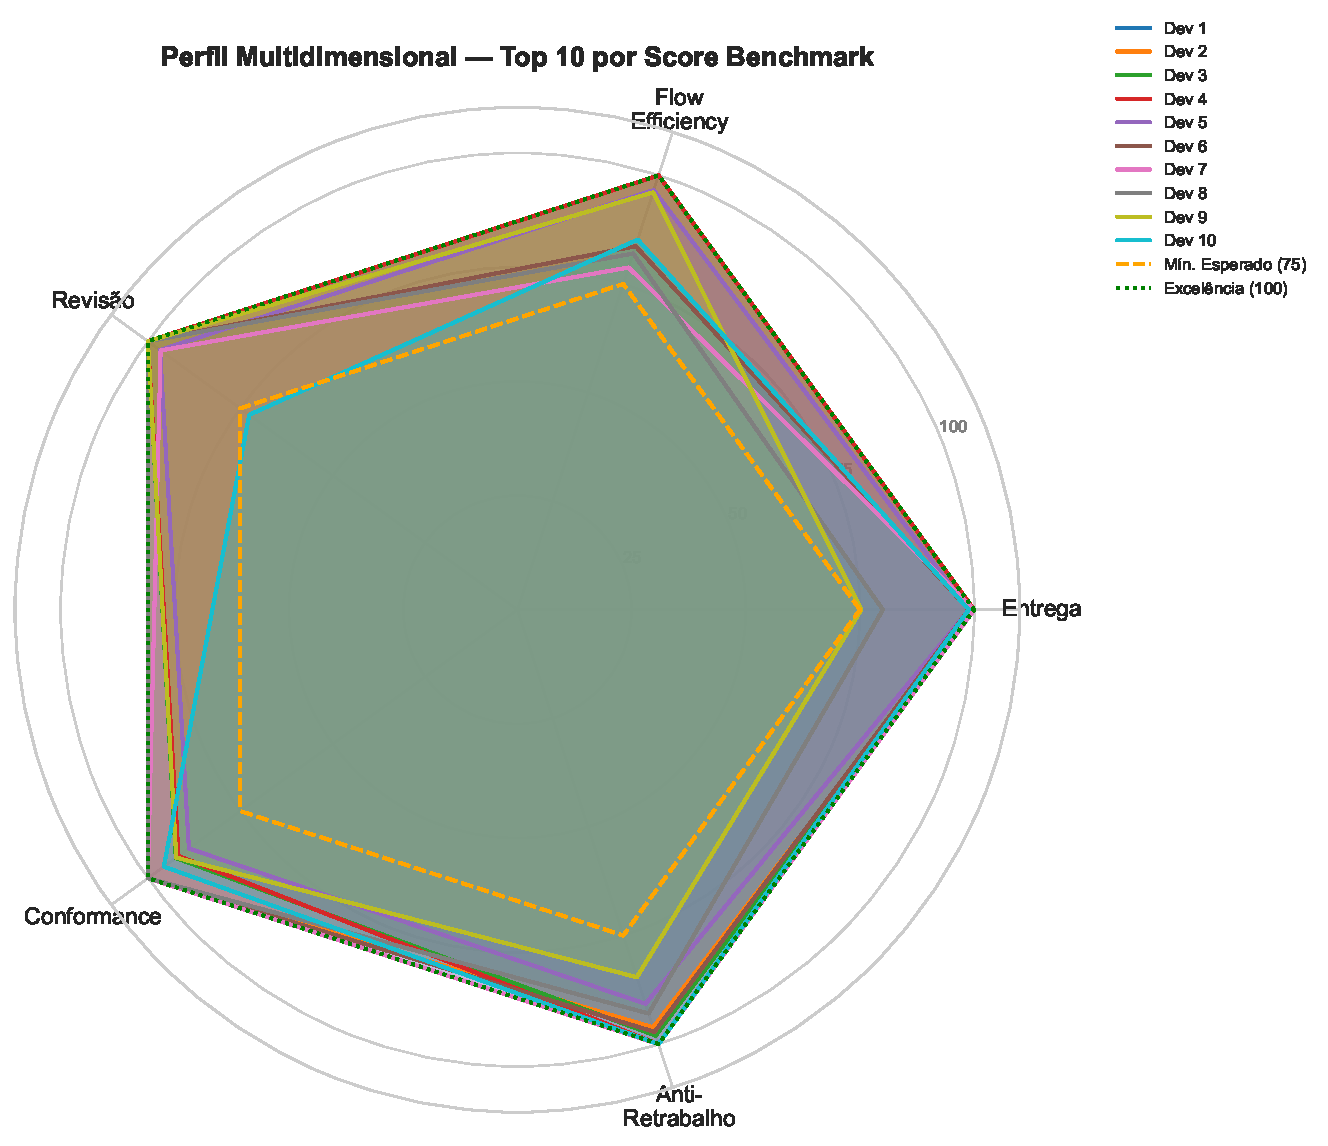
\includegraphics[width=0.95\columnwidth]{figures/fig1_radar.pdf}
  \caption{Radar chart of the five normalized dimensions for the top 10 developers
    by Score Benchmark (Q3~2024, $n=28$, seed=42). Orange dashed: minimum expected
    (75); green dotted: excellence (100). The Delivery dimension shows the widest
    variance (CV~$=0.46$); Anti-Rework and Review Quality cluster near 90+.}
  \label{fig:radar}
\end{figure}

\subsection{Flow Efficiency and Process Quality (RQ2)}

The Pearson correlation between FE and Conformance Quality is $r=0.15$
($p=0.44$), weak in the aggregate. However, developers with WIP~Residual~$>4$
items ($n=17$) exhibit mean FE of 61.9\% vs.\ 79.7\% for the low-WIP group
($n=11$) --- a 17.8~pp gap consistent with Little's Law~\cite{anderson2010}.
Rework acts as a common cause: all developers with rework rates exceeding 25\%
appear in the low-FE, low-Conformance quadrant of Figure~\ref{fig:scatter}.

\begin{figure}[htbp]
  \centering
  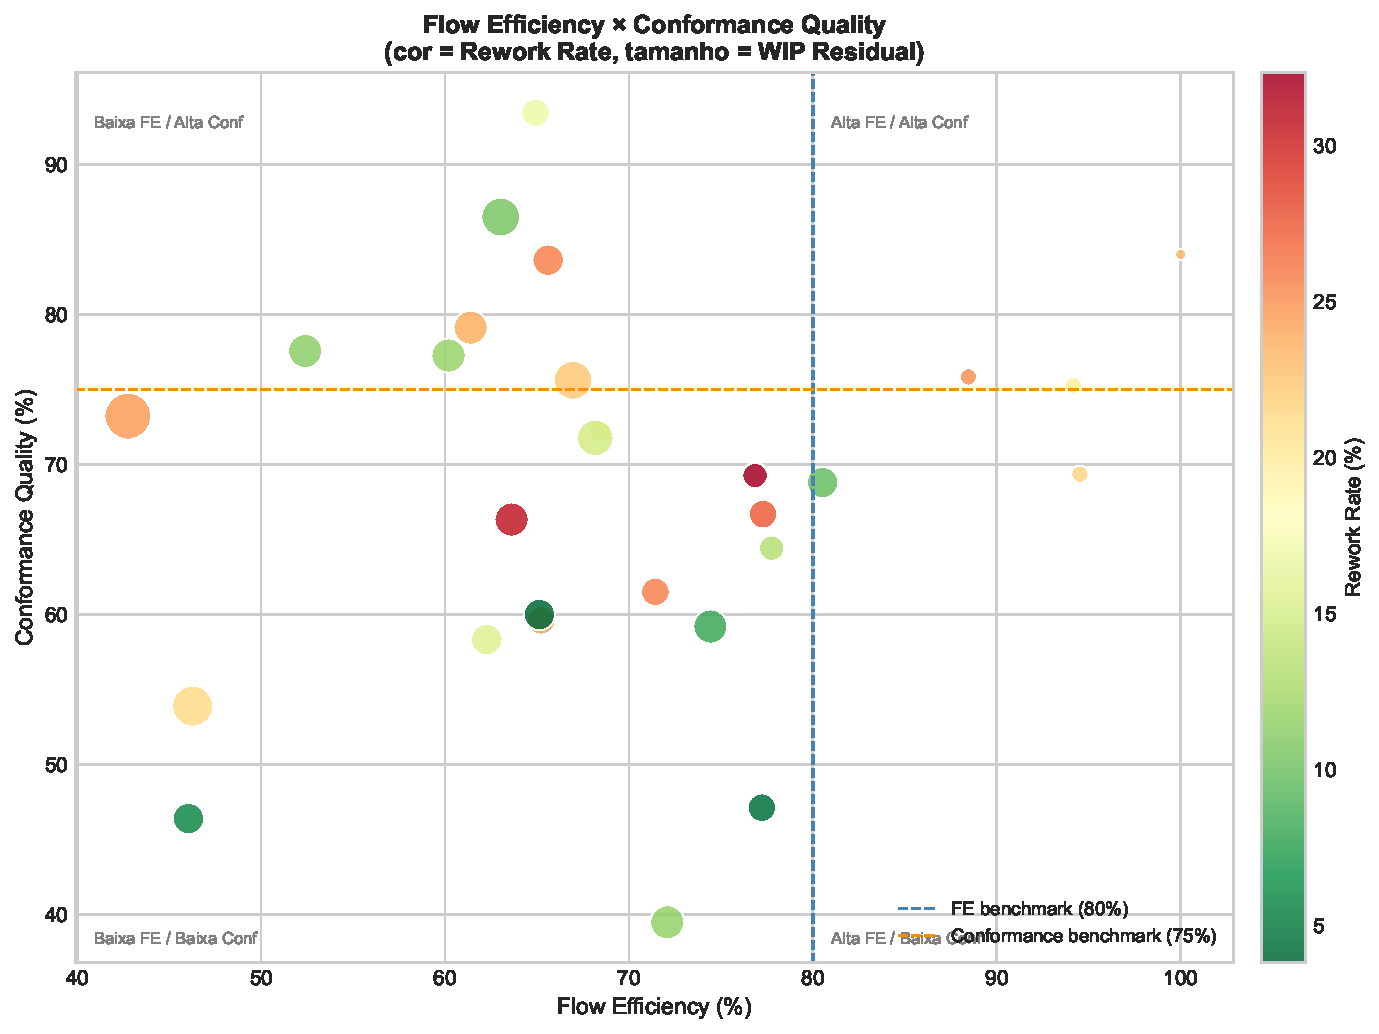
\includegraphics[width=0.95\columnwidth]{figures/fig2_scatter.pdf}
  \caption{Flow Efficiency vs.\ Conformance Quality. Bubble size $\propto$ WIP
    Residual; color encodes Rework Rate (blue = low, red = high). Dashed lines:
    benchmarks (80\%, 75\%). High-WIP developers cluster in the lower-left quadrant
    with elevated rework.}
  \label{fig:scatter}
\end{figure}

\subsection{Role-Fair NDS Benchmarking (RQ3)}

Table~\ref{tab:role_correction} quantifies the NDS and IED correction from
role-specific P75 benchmarking (Dev~P75~$=23.0$; TL~P75~$=13.0$).

\begin{table}[htbp]
  \centering
  \caption{NDS and IED by role: global vs.\ role-specific P75.}
  \label{tab:role_correction}
  \small
  \setlength{\tabcolsep}{4pt}
  \begin{tabular}{lcccccc}
    \toprule
    & \multicolumn{3}{c}{\textbf{Global P75 = 21.25}} & \multicolumn{3}{c}{\textbf{Role P75}} \\
    \cmidrule(lr){2-4}\cmidrule(lr){5-7}
    & Dev & TL & Gap & Dev & TL & Gap \\
    \midrule
    NDS  & 89.4 & 47.1 & $-42.3$ & 82.6 & 76.9 & $-5.7$ \\
    IED  & 77.9 & 61.0 & $-16.9$ & 76.4 & 72.1 & $-3.7$ \\
    IEF  & 78.3 & 51.4 & $-26.9$ & 75.6 & 70.7 & $-4.9$ \\
    \bottomrule
  \end{tabular}
\end{table}

With global P75, the mean TL NDS is 47.1 --- structural disadvantage, not
underperformance. Role-specific P75 narrows the NDS gap from $-42.3$ to $-5.7$~pp
and the IED gap from $-16.9$ to $-3.7$~pp (\textbf{RQ3}). The residual $-3.7$~pp
IED gap is attributable to VEL (TL median LT 4.91 vs.\ Dev 4.29~days) and
the lower Conformance noted in Table~\ref{tab:desc}.

\begin{figure}[htbp]
  \centering
  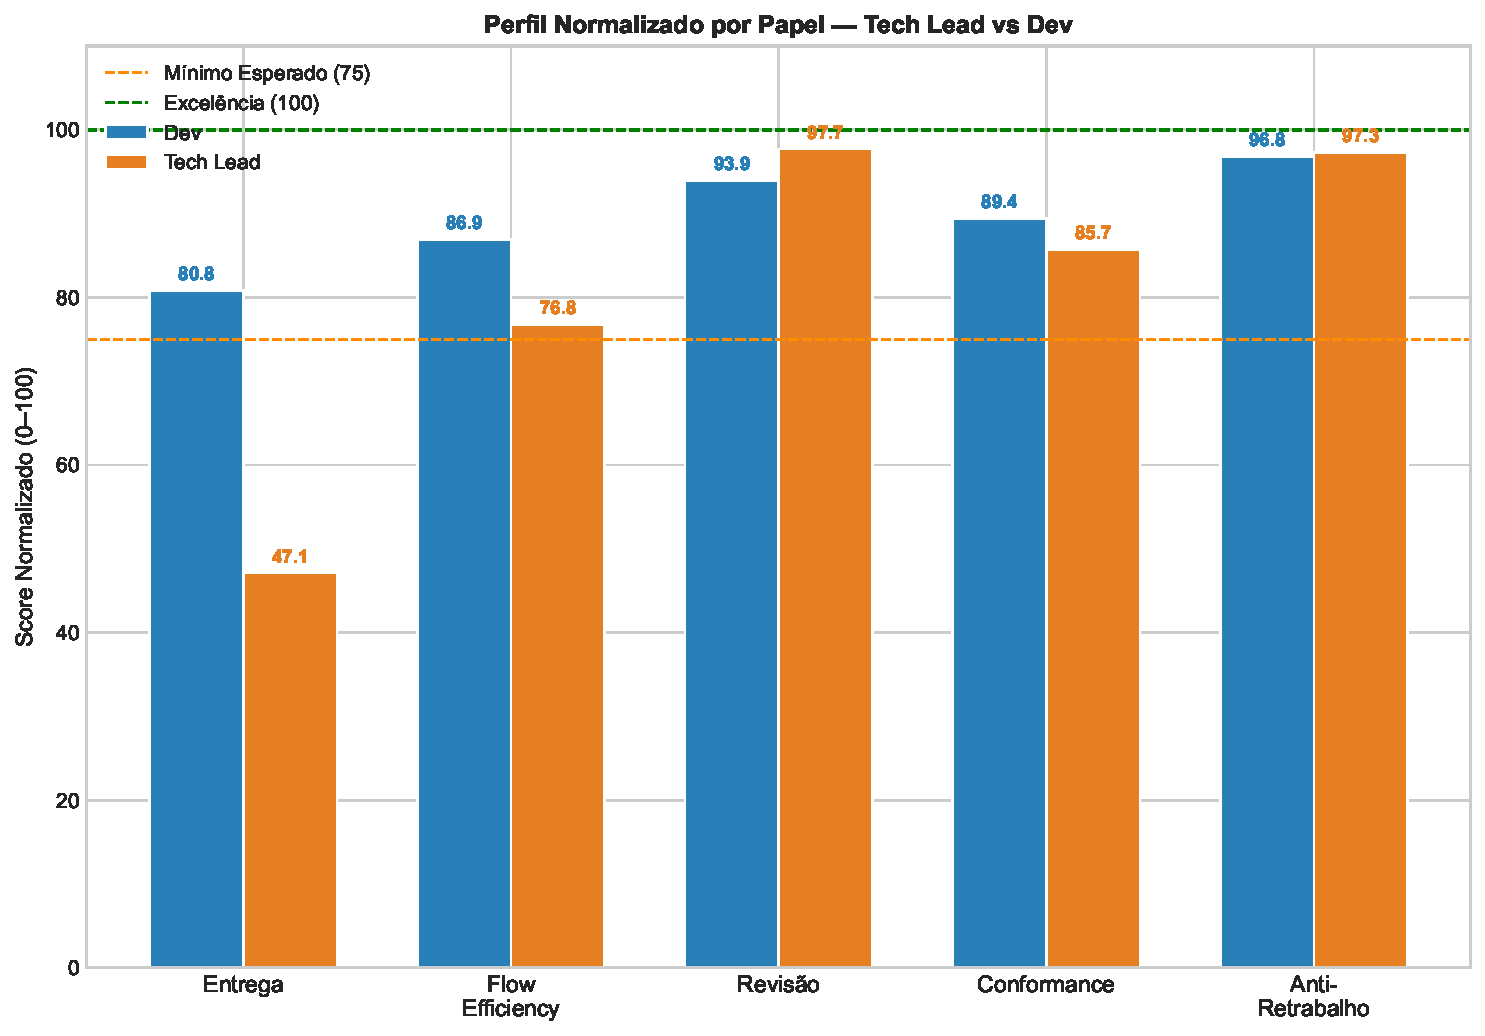
\includegraphics[width=0.95\columnwidth]{figures/fig4_role_bars.pdf}
  \caption{Normalized dimension scores: Dev (blue) vs.\ Tech Lead (orange). The
    Delivery ($-42.3$~pp with global P75) is the dominant penalty; Review Quality
    and Anti-Rework favor Tech Leads.}
  \label{fig:rolebars}
\end{figure}

\subsection{IEF--IED Divergence as Diagnostic Signal (RQ4)}

Three developers exhibit $|\Delta| > 15$ under role-specific NDS
(Table~\ref{tab:divergence}).

\begin{table}[htbp]
  \centering
  \caption{Developers with IEF--IED divergence $\Delta > 15$.}
  \label{tab:divergence}
  \small
  \setlength{\tabcolsep}{3pt}
  \begin{tabular}{lcccclp{2.6cm}}
    \toprule
    Dev & Team & IEF & IED & $\Delta$ & Dir. & Root Cause \\
    \midrule
    DEV006 & W1NNER & 46.9 & 65.1 & 18.2 & $<$ & VEL=100, QUA=100; IED boosted by process despite low NDS/EEE \\
    DEV009 & W1NNER & 92.3 & 76.7 & 15.6 & $>$ & VEL=21.7 (LT=21.4d vs.\ median 4.7d); throughput masked by slow cycle \\
    DEV021 & BeFinance & 57.0 & 72.5 & 15.5 & $<$ & VEL=100; IED elevated by speed despite low NDS \\
    \bottomrule
  \end{tabular}
\end{table}

\textbf{DEV009} is the canonical IEF $>$ IED case: Score~Complexity~$=24$,
FE~$=74.4\%$ --- strong throughput --- but LT~$=21.4$~days yields
VEL~$=21.7$, pulling IED to 76.7. The coaching intervention is cycle-time
reduction (smaller batches, WIP limits), not delivery volume.
\textbf{DEV006} illustrates the opposite: IEF~$<$~IED because VEL and QUA inflate
the composite above the delivery signal. The manager relying on IED alone would
assign a positive coaching message; IEF ($=46.9$, low NDS) reveals the correct
picture (\textbf{RQ4}).

\subsection{Score Benchmark Distribution}

Figure~\ref{fig:hist} shows the SB distribution: median~80.2, left-skewed, mode
bin $[70,80)$. The weakest normalized dimension is Delivery (mean~72.4), followed
by Flow Efficiency (mean~84.4). Anti-Rework (96.9) and Review Quality (94.8) are
near-ceiling, confirming that delivery throughput and WIP discipline --- not
process quality --- are the primary improvement levers in this cohort.

\begin{figure}[htbp]
  \centering
  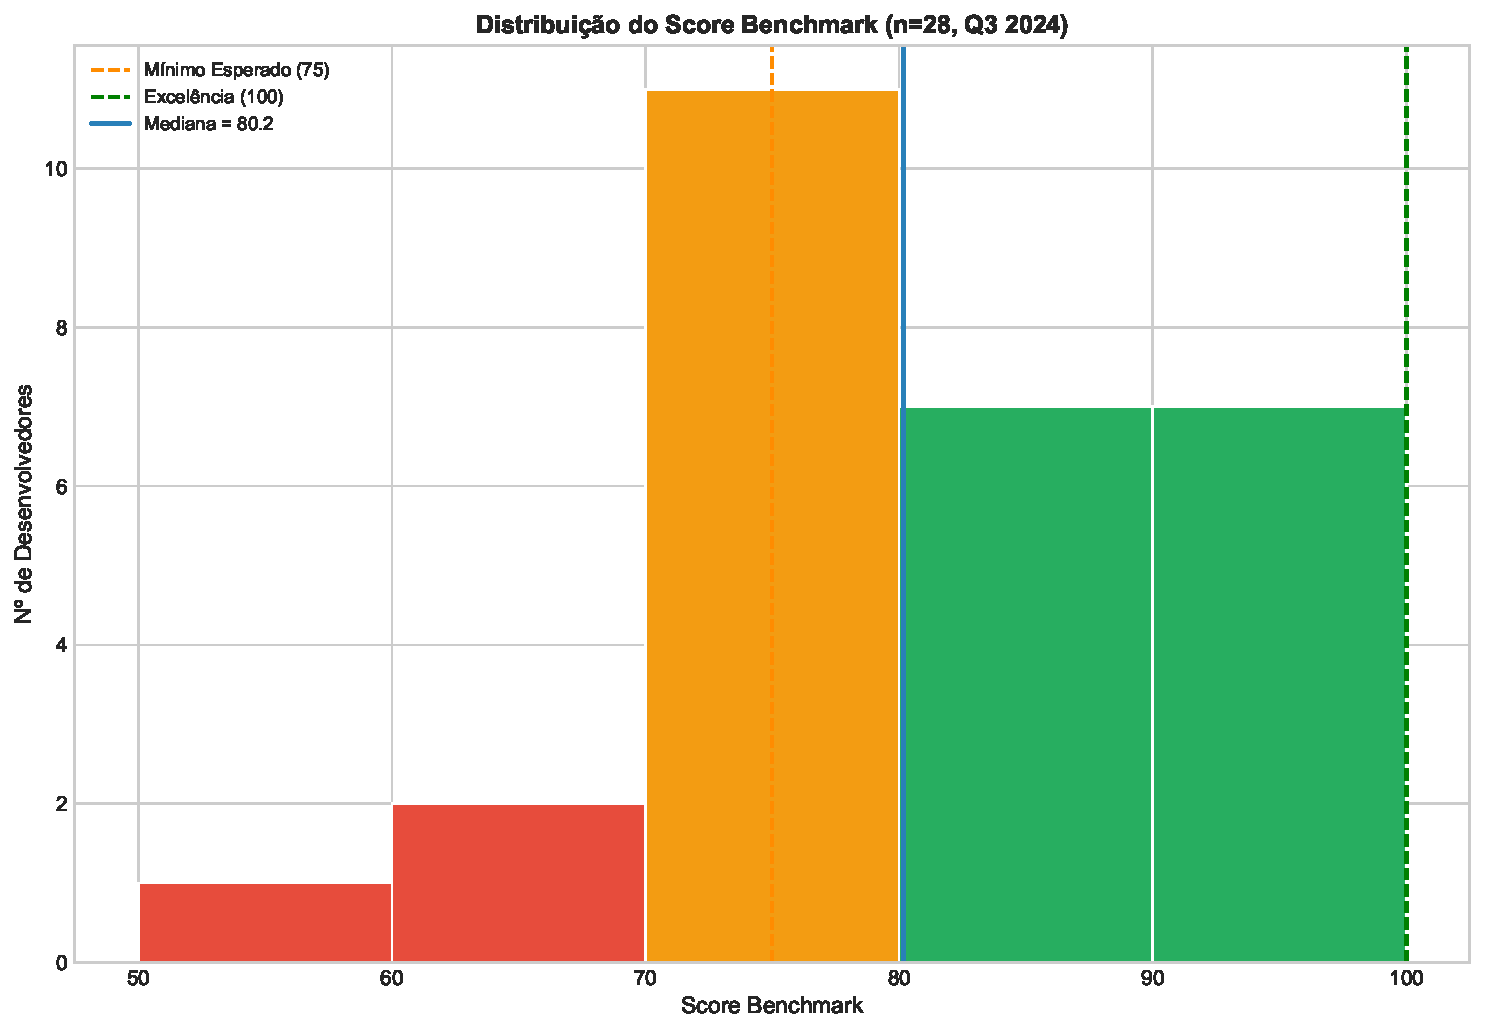
\includegraphics[width=0.95\columnwidth]{figures/fig3_histogram.pdf}
  \caption{Score Benchmark distribution (all 28~developers, Q3~2024, seed=42).
    Red: below 75; orange: 75--85; green: above 85. Dashed lines: minimum
    expected (75) and excellence (100). Median: 80.2.}
  \label{fig:hist}
\end{figure}

\subsection{QUA Bayesian Smoothing Effects}

The correction is negligible for $\geq 15$~deliveries ($|\Delta\text{QUA}|<3$~pp)
but substantial for low-sample cases. Table~\ref{tab:bayes} reports the five
largest corrections in the synthetic cohort.

\begin{table}[htbp]
  \centering
  \caption{QUA correction from Bayesian smoothing ($\alpha=0.5$, $\beta=9.5$).}
  \label{tab:bayes}
  \small
  \setlength{\tabcolsep}{4pt}
  \begin{tabular}{lcccccc}
    \toprule
    Dev & Del. & Def. & QUA$_\text{raw}$ & QUA$_\text{bayes}$ & $\Delta$QUA & $\Delta$IED \\
    \midrule
    DEV024 & 7  & 6 & 14.3 & 61.8 & +47.5 & +4.75 \\
    DEV025 & 7  & 3 & 57.1 & 79.4 & +22.3 & +2.23 \\
    DEV026 & 8  & 3 & 62.5 & 80.6 & +18.1 & +1.81 \\
    DEV023 & 9  & 3 & 66.7 & 81.6 & +14.9 & +1.49 \\
    DEV010 & 4  & 1 & 75.0 & 89.3 & +14.3 & +1.43 \\
    \bottomrule
  \end{tabular}
\end{table}

DEV024 (6~defects in 7~deliveries) illustrates the problem: raw QUA~$=14.3$
classifies this developer as ``Critical'' on quality, inflating the IED penalty
by $0.10 \times 47.5 = 4.75$~points. The Bayesian estimate of 61.8 is
statistically defensible for a sample of~7 while still indicating elevated
failure demand. The raw QUA column is retained for audit purposes.

\subsection{ICC --- Commit Concentration per Team}

Table~\ref{tab:icc} reports ICC for all five teams.

\begin{table}[htbp]
  \centering
  \caption{ICC (Herfindahl-Hirschman) per team.}
  \label{tab:icc}
  \small
  \begin{tabular}{lcrrrp{1.8cm}}
    \toprule
    Team & $N$ & Commits & ICC & ICC$_\text{norm}$ & Class \\
    \midrule
    W1NNER    & 9 & 484 & 0.122 & 0.012 & Distributed \\
    S1NC      & 7 & 445 & 0.167 & 0.028 & Distributed \\
    BeFinance & 5 & 233 & 0.271 & 0.089 & Moderate    \\
    Data      & 4 & 222 & 0.271 & 0.029 & Distributed \\
    Infra     & 3 & 149 & 0.362 & 0.043 & Distributed \\
    \bottomrule
  \end{tabular}
\end{table}

Raw HHI $> 0.25$ for Infra and Data appears alarming, but
ICC$_\text{norm}$ reveals it is a team-size artifact (minimum
$1/N = 0.33$ for $N=3$). BeFinance has the highest normalized concentration
(0.089), driven by one developer contributing 39.5\% of team commits --- a
bus-factor risk warranting cross-training investment.

\subsection{Empirical Production Results}

\begin{table}[htbp]
  \centering
  \caption{Anonymized production descriptives by team-quarter. Cells with $n < 5$ were merged into \texttt{Other}.}
  \label{tab:empirical-desc}
  \scriptsize
  \begin{tabular}{llrrrrrrrrr}
    \toprule
    Quarter & Team & $n$ & Delivered & Pulled & LT$_{50}$ & FE & Conf & Rework & Git & SB \\
    \midrule
    Q1-2025 & Team A & 15 & 135 & 243 & 14.0 & 55.6 & 50.7 & 0.0 & 48.9 & 63.8 \\
    Q2-2025 & Team A & 15 & 310 & 272 & 38.0 & 100.0 & 54.5 & 29.6 & 41.0 & 68.2 \\
    Q3-2025 & Team A & 16 & 455 & 409 & 29.5 & 100.0 & 64.8 & 0.0 & 45.9 & 70.3 \\
    Q4-2025 & Team A & 16 & 383 & 387 & 9.0 & 99.0 & 63.5 & 0.0 & 32.4 & 66.1 \\
    \bottomrule
  \end{tabular}
\end{table}

\small
% Auto-generated by paper/generate_empirical_validation.py
Empirical validation used 4 anonymized team-quarter observations across 1 published cohorts. Inclusion required complete Jira, Bitbucket, and process-mining coverage for the analyzed window.

Benchmark attainment was strongest for Anti-Rework (100.0\% of team-quarter observations at or above target) and weakest for Conformance (0.0\%).

High-WIP cohorts showed a median lead-time penalty of 6.8 days and a median rework penalty of 14.8 percentage points relative to low-WIP cohorts, supporting the flow-health interpretation of WIP residual.

\normalsize

\begin{figure}[htbp]
  \centering
  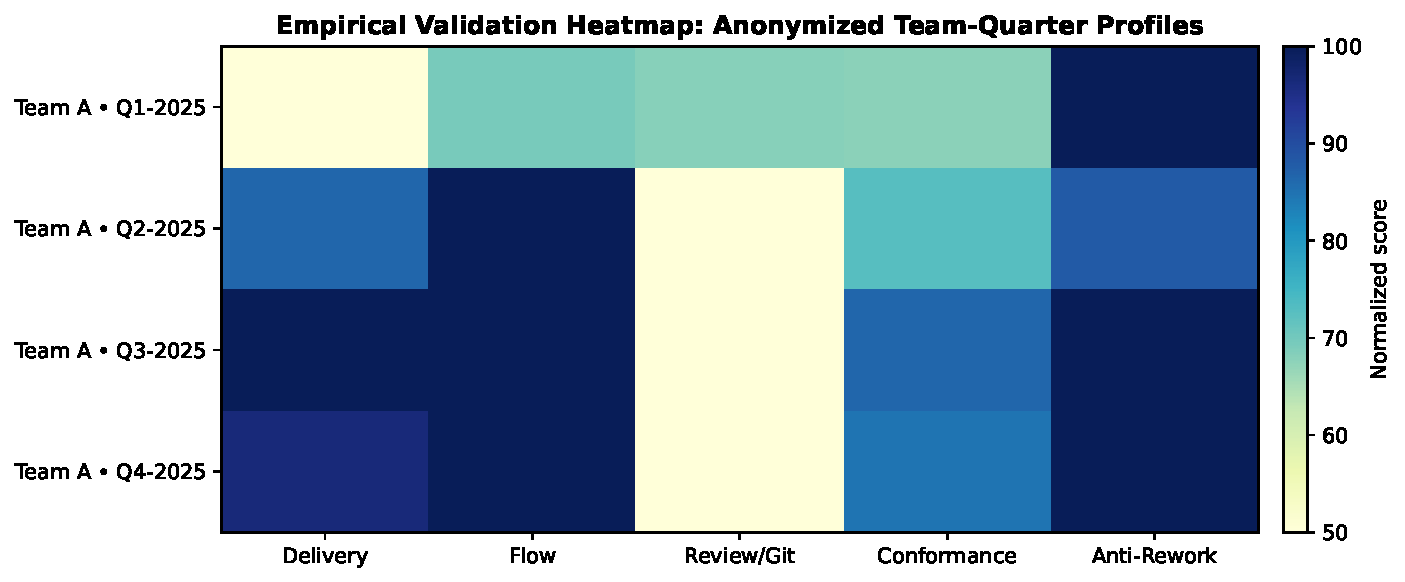
\includegraphics[width=0.95\columnwidth]{figures/fig5_empirical_heatmap.pdf}
  \caption{Heatmap of anonymized team-quarter profiles in the empirical validation.
    Multiple cohorts can appear simultaneously above or below benchmark, avoiding
    the artificial winner-loser ordering of relative normalization.}
  \label{fig:heatmap}
\end{figure}

\begin{figure}[htbp]
  \centering
  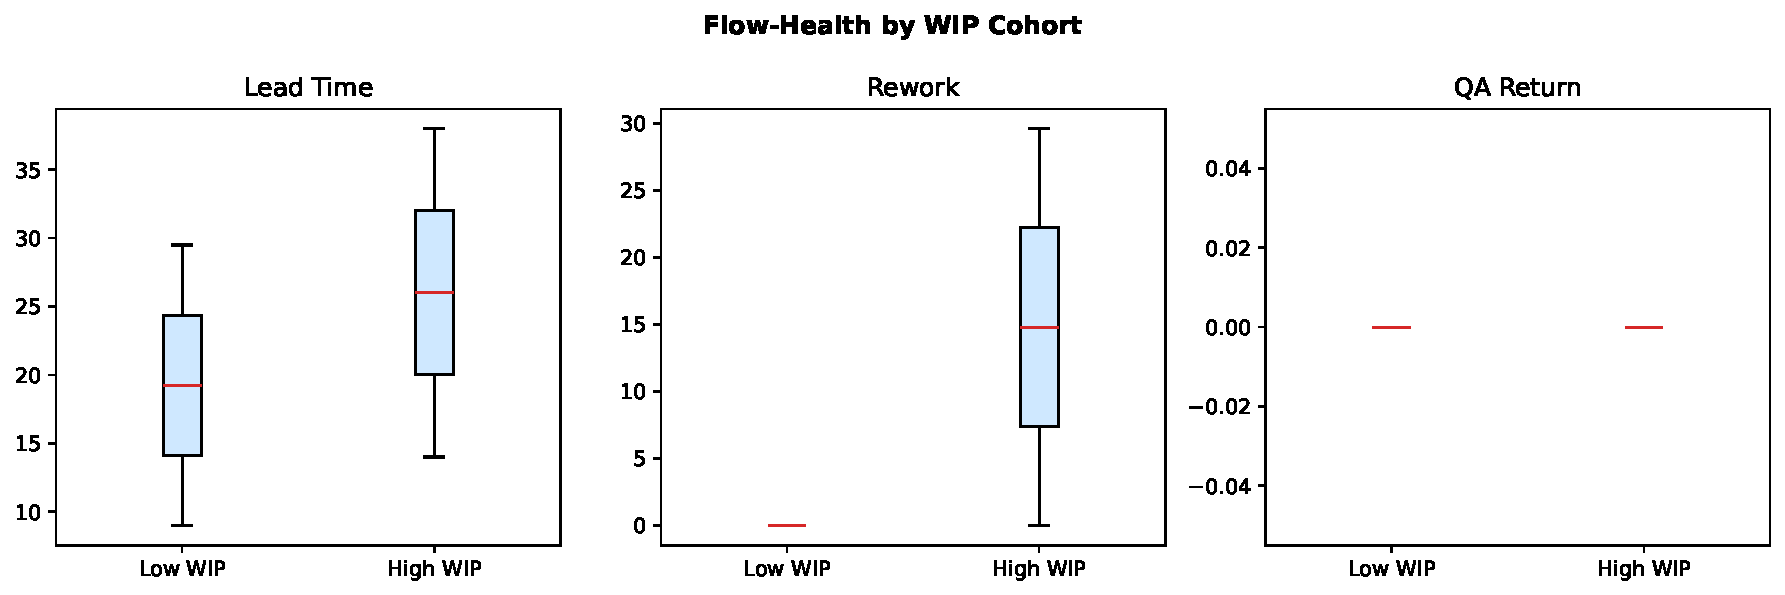
\includegraphics[width=0.95\columnwidth]{figures/fig7_wip_boxplot.pdf}
  \caption{Lead time, rework, and QA return distributions for low-WIP vs.\
    high-WIP anonymized cohorts. High-WIP cohorts exhibit systematically worse
    behavior on all three process-health signals.}
  \label{fig:wip}
\end{figure}

% ============================================================
\section{Threats to Validity}
\label{sec:threats}
% ============================================================

\paragraph{Construct validity.}
Metrics are proxies for latent productivity constructs~\cite{kitchenham1995}.
IED and IEF component weights (0.40/0.30/0.20/0.10 and 0.70/0.30) are
theoretically motivated but empirically unvalidated.

\paragraph{Internal validity.}
The evaluation uses synthetic data. Correlations in Section~\ref{sec:results}
are plausible but not necessarily representative. The Bayesian prior
($\alpha=0.5$, $\beta=9.5$) is fixed and not calibrated to the evaluation cohort.

\paragraph{External validity.}
FlowPMO assumes Jira + Bitbucket. Organizations using GitHub, GitLab, or Azure
DevOps require adapter development. Benchmarks (FE~$\geq 80\%$, Conformance
$\geq 75\%$) may not generalize to domains with longer approval cycles
(e.g., embedded systems, regulated industries).

\paragraph{Conclusion validity.}
SB assigns equal dimension weights; IED assigns fixed component weights. Neither
is empirically validated. Euclidean distance treats all shortfalls symmetrically.
Weighted calibration via Analytic Hierarchy Process is the highest-priority future
work item.

\paragraph{Privacy and disclosure.}
The production study suppresses small groups and removes raw identifiers, reducing
re-identification risk but also attenuating statistical power. Some signal
attenuation is an accepted trade-off of privacy-preserving reporting.

% ============================================================
\section{Discussion}
\label{sec:discussion}
% ============================================================

\subsection{Absolute vs.\ Relative Normalization}

Preliminary experiments showed that z-score normalization on a 5-developer pilot
team assigned near-zero scores to all developers on the Delivery dimension despite
Score~Complexity values ranging from 8 to~26. Absolute normalization preserves the
external referent: a developer scoring $\hat{d}_\text{flow}=60$ is at 60\% of the
Anderson~\cite{anderson2010} benchmark regardless of peer performance.

The role-specific P75 extension introduces a limited within-role relative
reference for D1 while retaining absolute external validity for all other
dimensions. Future work should explore whether role-specific absolute benchmarks
can be derived from industry surveys.

\subsection{IED and IEF as Coaching Instruments}

The three divergence cases (Table~\ref{tab:divergence}) illustrate two coaching
failure modes that are invisible in either index alone:

\begin{enumerate}
  \item \textbf{IEF $>$ IED (VEL penalty)}: high throughput masked by long cycle
    time. Coaching intervention: batch size reduction, WIP limits.
  \item \textbf{IEF $<$ IED (process bonus)}: excellent speed or quality inflates
    IED above delivery capacity signal. Coaching intervention: focus on
    throughput.
\end{enumerate}

$\Delta > 15$ flags the 10--15\% of developers where IEF and IED give
materially different coaching directions. For the remaining 85--90\%
($|\Delta| \leq 15$), both indices are sufficiently aligned.

\subsection{Bayesian Shrinkage and Small-Sample Scoring}

The QUA correction results highlight a broader principle: any rate-based metric
with a denominator below $\approx 15$ is a poor estimator of the underlying rate.
A Beta-Binomial prior is the principled solution. In principle, EEE and even
NDS are susceptible to similar instability in very small cohorts; future work
should explore Bayesian formulations for all sub-indices.

\subsection{ICC as Organizational Risk Signal}

Raw HHI is misleading across teams of different sizes (Table~\ref{tab:icc}).
ICC$_\text{norm}$ corrects for this. Organizations with many small teams may need
role-adjusted ICC variants that account for expected contribution asymmetries
(e.g., TLs commit less structurally). An ICC$_\text{norm}$ rising across
consecutive quarters in the same team, combined with the existing KCR
(Knowledge Concentration Risk) truck-factor indicator, provides a stronger
basis for cross-training decisions than either signal alone.

% ============================================================
\section{Conclusion}
\label{sec:conclusion}
% ============================================================

This paper presented FlowPMO, an open-source framework for multidimensional
developer productivity measurement. Beyond the original five SPACE-inspired
dimensions and Score Benchmark, the extended framework introduces IED, IEF,
IEF--IED Divergence, role-fair NDS benchmarking, Bayesian QUA smoothing,
FE~Ajustada, ECR badge, and team-level ICC --- collectively addressing eight
measurement validity threats identified in the literature and in production
deployment.

Key findings on the synthetic cohort:

\textbf{RQ1}: Commit count correlates weakly with SB ($r=0.36$) and IED
($r=0.31$). The multidimensional composite captures variance invisible to single
metrics, illustrated by two developers differing by 9.9~SB points despite
similar commit counts.

\textbf{RQ2}: WIP accumulation is a strong moderating variable: high-WIP
developers exhibit FE 17.8~pp lower than low-WIP peers; rework acts as a common
cause of both low FE and low Conformance.

\textbf{RQ3}: Role-specific P75 reduces the NDS gap from $-42.3$ to $-5.7$~pp
and the IED gap from $-16.9$ to $-3.7$~pp, qualitatively changing the coaching
signal for 7 of 28~developers.

\textbf{RQ4}: IEF--IED divergence exceeds 15~points for 3 of 28 developers
(10.7\%), each representing a distinct coaching scenario. DEV009's high-throughput
profile masked by long cycle time and DEV006's low-delivery profile inflated by
excellent process metrics both go undetected without the Divergence signal.

Complementary: Bayesian smoothing produces corrections up to 47.5~pp for
extreme low-sample cases; BeFinance has the highest normalized commit
concentration (ICC$_\text{norm}=0.089$), warranting cross-training investment.

\textbf{Future work} will pursue: (i)~empirical calibration of IED/IEF component
weights via longitudinal data and Analytic Hierarchy Process; (ii)~adapters for
GitHub, GitLab, and Azure DevOps; (iii)~organization-specific Bayesian prior
calibration from rolling defect-rate history; (iv)~longitudinal evaluation of
FE~Ajustada with real cross-period WIP data; (v)~SPACE Satisfaction dimension
integration via pulse-survey proxies.

% ============================================================
% REFERENCES
% ============================================================

\bibliographystyle{IEEEtran}

\begin{thebibliography}{19}

\bibitem{demarco1999}
  T.~DeMarco and T.~Lister,
  \textit{Peopleware: Productive Projects and Teams}, 2nd~ed.
  Dorset House, 1999.

\bibitem{forsgren2021}
  N.~Forsgren et~al.,
  ``The SPACE of Developer Productivity,''
  \textit{ACM Queue}, vol.~19, no.~1, pp.~20--48, 2021.

\bibitem{kitchenham1995}
  B.~Kitchenham, S.~L.~Pfleeger, and N.~Fenton,
  ``Towards a Framework for Software Measurement Validation,''
  \textit{IEEE TSE}, vol.~21, no.~12, pp.~929--944, 1995.

\bibitem{anderson2010}
  D.~J.~Anderson,
  \textit{Kanban: Successful Evolutionary Change for Your Technology Business}.
  Blue Hole Press, 2010.

\bibitem{shah2023}
  S.~M.~A.~Shah et~al.,
  ``An Empirical Study on the Relationship Between Rework and Technical Debt,''
  in \textit{Proc.\ ICSME}, 2023, pp.~1--12.

\bibitem{caldeira2019}
  J.~Caldeira et~al.,
  ``Conformance Quality in Software Development: A Process Mining Approach,''
  in \textit{Proc.\ ICPM}, 2019, pp.~121--128.

\bibitem{fenton1997}
  N.~Fenton and S.~L.~Pfleeger,
  \textit{Software Metrics: A Rigorous and Practical Approach}, 2nd~ed.
  PWS Publishing, 1997.

\bibitem{jorgensen2014}
  M.~J{\o}rgensen,
  ``What We Know About Software Development Effort Estimation,''
  \textit{IEEE Software}, vol.~31, no.~2, pp.~37--40, 2014.

\bibitem{forsgren2018}
  N.~Forsgren, J.~Humble, and G.~Kim,
  \textit{Accelerate}.
  IT Revolution Press, 2018.

\bibitem{vanderaalst2016}
  W.~M.~P.~van der Aalst,
  \textit{Process Mining: Data Science in Action}, 2nd~ed.
  Springer, 2016.

\bibitem{caldeira2021}
  J.~Caldeira et~al.,
  ``Mining Software Development Rework Patterns Using Process Mining,''
  \textit{Inf. Softw. Technol.}, vol.~135, p.~106565, 2021.

\bibitem{nogueira2023}
  A.~F.~Nogueira and M.~Z.~Rela,
  ``Continuous Integration Pipeline Quality,''
  \textit{Inf. Softw. Technol.}, vol.~161, p.~107256, 2023.

\bibitem{kitchenham2002}
  B.~Kitchenham,
  ``Procedures for Performing Systematic Reviews,''
  Keele Univ., Tech.~Rep.~TR/SE-0401, 2002.

\bibitem{gelman2013}
  A.~Gelman et~al.,
  \textit{Bayesian Data Analysis}, 3rd~ed.
  CRC Press, 2013.

\bibitem{ricca2019}
  C.~Ferme, N.~Leger, and N.~Anquetil,
  ``Who Is Going to Maintain This Code? Supporting Truck Factor Analysis,''
  in \textit{Proc.\ IWESEP}, 2019.

\bibitem{doj2010}
  U.S.~Dept.\ of Justice and FTC,
  \textit{Horizontal Merger Guidelines}, \S5.3, 2010.

\bibitem{kitchenham2004}
  B.~Kitchenham and E.~Mendes,
  ``A Comparison of Cross-Company and Within-Company Effort Estimation
  Models for Web Applications,''
  \textit{IEEE TSE}, vol.~30, no.~11, pp.~722--737, 2004.

\bibitem{flournoy2025}
  R.~Flournoy, C.~Treude, and B.~Adams,
  ``Cycle Time as a Proxy for Developer Productivity: An Empirical Study,''
  \textit{Empir. Softw. Eng.}, vol.~30, no.~2, 2025.

\end{thebibliography}

\end{document}
